\section{requirement specification}

\subsection{Overview}

\begin{itemize}
 \item provide status information to MAC
 \item switch states (RX, TX, SLEEP)
 \item send packets to air/channel
 \item receive packets / listen for packets
 \item provide hooks for statistical information
 \item configurable settings
\end{itemize}

\subsection{provide status information to MAC}

In addition to received packets the physical layer has to provide some other information
to the MAC layer.
Some of this information has to be provided passively on demand (e.g. current mode) and some should
be delivered actively to the MAC layer on certain events (e.g. transmission of a packet complete).

\noindent Information which has to be provided to MAC on demand:
\begin{itemize}
 \item current signal strength or SNR information on channel
 \item current mode (RX, TX, SLEEP)
 \item current channel
 \item other?
\end{itemize}

\noindent Information which has to be provided to MAC the moment it occurs:
\begin{itemize}
 \item transmission over (send)
 \item other?
\end{itemize}

\pagebreak
\subsection{switch states}

The physical layer has to be able to switch between the following things:

\begin{itemize}
 \item current mode (RX, TX, SLEEP)
 \item current channel (1, 2, 3, ...)
 \item other?
\end{itemize}

\begin{figure}[t]
 \centering
 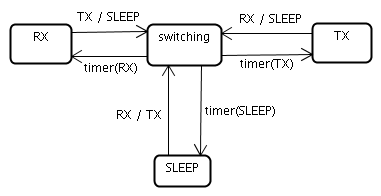
\includegraphics[width=240pt]{req_spec/stateMachineMode.png}
 % stateMachineMode.png: 1179666x1179666 pixel, 0dpi, infxinf cm, bb=
 \caption{State machine for current mode}
 \label{fig: mode state machine}
\end{figure}

\pagebreak
\subsection{send packets}

The physical layer has to be able to send packets from the MAC 
Layer to the channel.

Before we can send packets the following things have to be 
assured:
\linebreak
\begin{itemize}
 \item the radio has to be in TX mode
 \item we are not already sending
 \item the channel should be idle (maybe this is no hard requirement)
\end{itemize}

The above items should be controlled by the MAC-Layer so the physical layer 
would only throw an error if they are not set.

The sending process itself is made up of the following steps:

\begin{enumerate}
 \item MAC layer gives packet and control info to physical layer
 \item check requirements for sending, throw error if they are not fulfilled
 \item add information needed by the receiving physical layer to packet (see below)
 \item packet is send to channel by physical layer
\end{enumerate}

The following information is needed by the receiving physical layer:

\begin{itemize}
\item TX power
\item position, move direction and speed of the sending host
\item the channel
\item size of packet
\item the duration the signal would need to be transmitted
\item the bitrate (payload and header)

\end{itemize}

\subsection{receive packets}

Following things have to be done with every received packet:

\begin{enumerate}
 \item get transmission time of the packet and schedule transmission over event
 \item apply \textit{analog model} (simulate pathloss, shadowing, fading) to 
 			 calculate signal strength over time 
\end{enumerate}

Every packet has to be classified as 
\textit{signal}\footnote{We have some name collision here. With signal 
												 we mean every signal we receive over the channel. 
												 With \textit{signal} we mean the signal we try to 
												 receive as a packet.} 
or \textit{noise}. The decision depends on one or more of the following 
points.

\begin{itemize}
 \item signal strength (at signal start)
 \item are we already listening to a \textit{signal} (most time we won't be able to listen to more than one 
 			 \textit{signal} at the same time, so every thing else is \textit{noise})
\end{itemize}

If the transmission of a \textit{signal} is over we have to decide if it was received correctly. This is
done with a \textit{demodulation module} by evaluating the \textit{signal to noise ratio} short \textit{SNR}. If the signal was received correctly pass it (together with its SNR information) to the MAC Layer.

\subsubsection{the analog model}

The \textit{analog model} has to be able to simulate the following things:

\begin{itemize}
 \item pathloss
 \item shadowing
 \item fading
\end{itemize}

Further we set the following requirements to the \textit{analog model}:

\begin{itemize}
 \item physical layer should be able to apply multiple \textit{analog models} to a signal
 \item you should be able to set the \textit{analog models} independent from physical layer
 \item you should be able to add your own \textit{analog models}
\end{itemize}

\subsubsection{the demodulation module}

We set the following requirements to the \textit{demodulation module}:

\begin{itemize}
 \item you should be able to set the \textit{demodulation module} independent from physical layer
 \item you should be able to add your own \textit{demodulation module}
 \item the \textit{analog model} should be able to return bitwise correctness of the signal (on demand)
\end{itemize}


\subsection{statistical information}

You should be able to get the following statistical information (the physical layer should not evaluate them but has to provide access to the according information):

\begin{itemize}
 \item packet count
 \item received signal strength
 \item signal to noise ratio
 \item bit error ratio
 \item collisions
 \item other?
\end{itemize}

\subsection{parameters}

The following parameters of the physical layer should be freely configurable:

\begin{itemize}
\item simulate propagation delay? (boolean)
\item which analog models should be used
\item the parameters for the analog models
\item which demodulation module should be used
\item the parameters for the demodulation module
\item thermal noise
\item sensitivity
\item maximum TX power
\item switching times between modes (RX, TX, SLEEP)
\end{itemize}
